\section{Introduction}

%\begin{figure}[!t]
%\vskip -0.03in
%  \centering
%      {
%        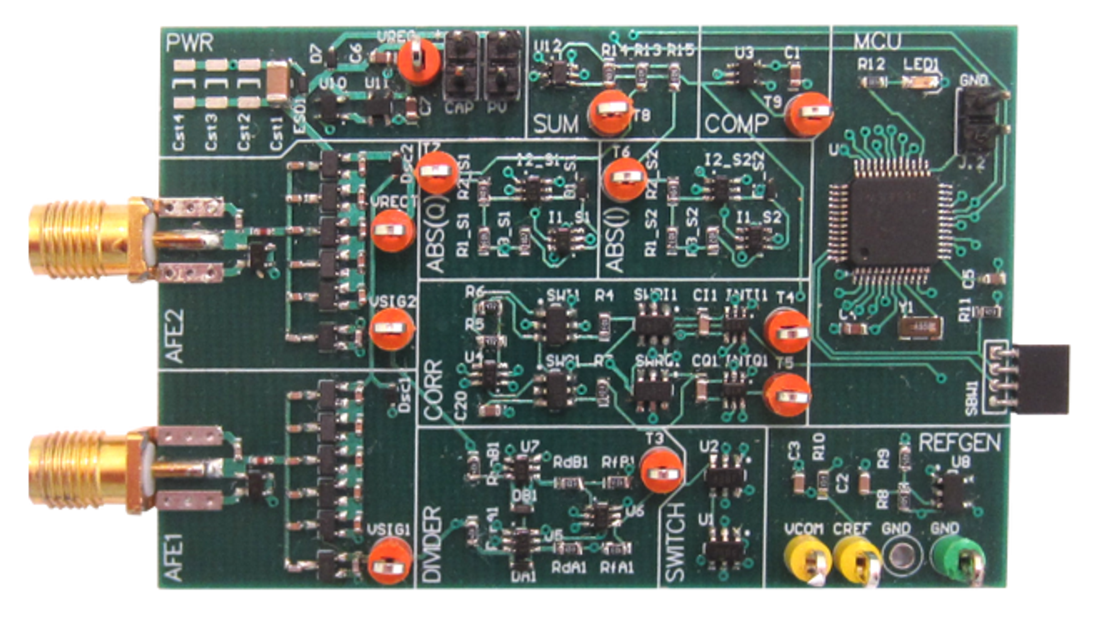
\epsfig{file=prototype-photo.eps, width=0.6\columnwidth}
%      }
%\caption{{\bf Our \vitag\ Prototype} \hl{integrates both mmm in a single design. It can operate using both RFID and TV transmissions}.}
%\label{fig:tag}
%\vskip -0.05in
%\end{figure}

%Due to the scarcity of radio spectrum, visible light communication (VLC) has attracted increasing research attention since the last decade due to the extra wide spectrum (i.e., from 400-800 THz) and the safety advantages of visible lights~\cite{expensive,expensive2,retro1,retro2,fundamental1, led2led1, standard}.  Significant results have been achieved, e.g.\, 3.8Gbps at 1m distance, 10Mbps at 10km using specialized devices and high power lights \cite{??,??}. A standard (IEEE 802.15.7) has been established recently~\cite{standard} to ensure inter-operation among devices from different manufacturers. 

%For illumination, white LEDs are commonly used. The instantaneous On/Off feature turns LEDs into effective transmitters for visible light communication (VLC). Specifically, information bits can be embedded on the light by modulating the on/off state of the LED with on-off keying (OOK) or variable pulse-position modulation (VPPM) \cite{standard}. To receive such signals, while in some cases a cell phone camera or a digital camera will be sufficient \hl{need citations, ipsn14 and mobicom14}, photodiodes are generally used, because phone cameras can only achieve around 0.25MHz sampling rate~\cite{camera1} (in other words, low data rate), whereas photodiodes have generally higher bandwidth up to 0.5GHz~\cite{pdsheet}. Moreover, compared with a phone camera, the SNR of the photodiode is orders of magnitude higher at the same distance \hl{ipsn14}. 

%A typical way to generate white lights is to use a phosphor material to convert monochromatic lights from blue or ultraviolet to broad-band white lights, where the color of the monochromatic light depends on the band gap energy of the materials forming the p-n junction in the LED. 


Nowadays, white LEDs have been prevalently deployed for illumination purpose for its advantageous properties such as high energy efficiency, long lifetime, environment friendliness, to name a few. Being semiconductor devices, LEDs also possess another feature, i.e.\, it can be turned on and off \textit{instantaneously}. This effectively turns LED lights into a carrier and gives rise to a new ''dual-paradigm'' -- illumination and communication. 
The ubiquity of lighting infrastructure makes this dual-paradigm VLC (i.e., communication over existing lighting infrastructure) especially well suited to communicate with mobile devices or sensor nodes, e.g., streaming video to one's mobile phone or to collecting environment data from home sensors. 

For any communication system or link, it is essential to have bi-directional communication capability to ensure reliability and flexibility. A minimum requirement would be able to acknowledge correct or incorrect receiving of packets. To realize bi-directional communication, a straightforward way is to put together two one-way communication links. Unlike existing radio communication systems where the radio front-end is shared for both transmitting and receiving, a VLC system uses an LED for transmitting and use a light sensor (e.g., photodiode) for receiving. In consequence, existing work on VLC has primarily focused on improving the throughput for one-way link using power hungry, expensive, and dedicated devices \cite{expensive,expensive2,retro1,retro2}.  

However, the dual-paradigm nature of the system, with illumination being the primary goal, naturally leads to an asymmetric communication setting. On the one end is the externally powered LED, on the other end is the power-constrained device such as mobile phones and even weaker sensor nodes. Such an asymmetric setting makes it \textit{unfit} to symmetrically put two one-way communication links because the weak end cannot afford the power-intensive LED. Even if an LED were used, the glaring light would be very annoying to human eyes. In fact, some early VLC-based practical systems such as ByteLight~\cite{ble0}, which exploits LED lighting infrastructure for both communication and localization~\cite{location1,location2}, have adopted another medium (e.g., Bluetooth Low Energy (BLE)) for the device-to-LED communication, i.e., \textit{uplink}. This unfortunately incurs additional cost, bandwidth and system complexity. Also, the adoption of BLEs or LEDs for the uplink implies nearly omni-directional emissions, which accounts for extra power demand on the uplink. 
% A typical VLC link thus further includes intermediate optical components (e.g., lenses) for concentrating light. This leads to highly directional VLC systems and makes the actual design of a dual-paradigm VLC system deviate from those dedicated VLC systems aiming at extreme high data rate. 

In this paper, we present the design and implementation of \textit{\retro -- a low-power duplex VLC system}. Inspired by recent work on backscatter communication systems~\cite{abc1,abc4}, we avoid the usage of an LED for the uplink communication by backscattering the incoming light from the lighting LED. Central to \retro\ is the adoption of retro-reflecting material which can bounce back light of an arbitrary incidence angle \textit{along its incoming path}. This essentially forms an uplink that concentrates energy without other concentrating optical elements. We further modulate the reflected light by applying an LCD as a modulator. By tuning the translucence of the LCD, we control the passing of the light reflected by the retro-reflector, and encode information bits using On-Off-Keying (OOK). The modulated reflected light is then picked up by the photodiode on the LED side and decoded by a dedicated system.


%Enabling asymmetric low-power VLC communication is non-trivial. While the downlink is with powerful LEDs that can emit strong signals, the main challenge lies in the uplink. Applying existing LED-photodiode link straightforwardly to a mobile device or sensor node is not affordable. A typical VLC link consists of an LED, a photodiode and intermediate optical components (e.g., lenses). Existing work shows that one-way VLC link today can achieve bit rates up to $~10Mbps$ from an LED transmitter to a receiver over a distance of $~10km$~\cite{expensive,expensive2,retro1,retro2}. To achieve such high speeds, special and expensive hardware pieces such as multiple quantum well electro-absorption modulators and lasers have to be used~\cite{expensive}. Moreover, they consume orders of magnitude more power than is available on a low-power device. Using low-power LEDs \cite{} at tags seems a viable solution which however unfits our applications, which is detailed in Section~\ref{sec:proto}. 

%In this work, we propose a novel approach by toggling an \textit{LCD} to modulate a \textit{retro-reflector} directionally bouncing back the incoming light from the LED, which forms a low-power uplink. Our prototype is shown in Fig.~\ref{fig:tag}. By tuning the translucence of the LCD, we control the light perceived by the phtodiode at the LED side, encoding digital information using On-Off-Keying (OOK). The current consumed by the tag with a LCD modulator as well as a microcontroller is slightly above $200\mu A$. In other words, the tag can even be powered by a badge-size solar panel harvesting energy solely from the LED light. Downlink transmission is accomplished also in OOK with a LED bulb and a photodiode on the tag. Despite its low power consumption, designing such a system, however, is challenging for the following reasons:

%\note{liqul: These bullets are too low-level for ordinary reviewers. Make them more concise as well.}

To achieve low power consumption, we identify and overcome several challenges as follows: 1) power consumption of LCD; To push to the extreme the low power consumption; 2) weak signal detection at LED; 3) clock offset handling

% \begin{Itemize}
% \item Handling the high throughput LED-transmitted data is power consuming. 
% \item Transmitting with the LCD at a high toggling frequency consumes even more power than the receiver.
% \item The LED receiver must handle clock offsets from the mobile end with low clock oscillating frequency.
% \item The LED receiver has to detect retro-reflected signals 3 orders of magnitude weaker than interfering LED transmissions.  
% \end{Itemize}

%\note{liqul: put using BLE for upper-link communication into discussion.}

To address these challenges, we apply the following design principles:

\begin{itemize}
\item Use analog components over digital ones while achieving comparable accuracy; Design low-power amplifiers.
\item Recycle LCD energy. 
\item Avoid using crystal oscillators when transmitting.
\item Design algorithms to decode signals that suffer from severe clock offsets.
\end{itemize}

%\textbf{\retro.} To understand our \vitag\ design on battery-free ID card-sized tags, consider an LCD whose emitted light can be manipulated by an additional small circuit inside the light bulb. This circuit embeds information in the light and modulates it, while keeping the brightness of the light the same without any flickering. On the \vitag\ side, a light sensor captures the light signal that conveys information from the LED. To conserve energy, \vitag\ only uses analog components to demodulate the signal without an ADC. Upon detecting data, a low-power micro-controller on \vitag\ is waked up for uplink data transmission. It drives up the LCD to flicker, therefore sending data back to the LED by backscattering the light with a retro-reflector behind the LCD. This uplink data can be captured by a light sensor placed on the LED, along with interferences caused by downlink transmission, nearby human and object movements, household electricity fluctuations, and so on. A specifically designed receiver associated with the LED then performs the time recovery and demodulates the signal. To get a network of \vitag\/s and LEDs into play, we design a Media Access Control (MAC) protocol to mediate the communications in LEDs' illumination range. 

To demonstrate the effectiveness of \retro\ design, we implement a battery-free tag device, which operates by harvesting the energy of incoming light. The tag device is the same size of a credit card, one-third of the area is the retroreflector and two-thirds is the polycrystalline silicon solar cell. %\todo{describe the performance of the tag, e.g., working range, bit rate, etc.}
\figref{fig:system} depicts the tag.
We also explored the tradeoff between the solar panel area and the retro-reflector area for achieving a maximum working range in the worst case where the LED is the only light source, \ie no ambient light. %\todo{This suggests that the optimal value be a function of the solar cell efficiency and the reflecting concentration ratio.} 
\begin{figure}[th]
   \centering
   \includegraphics[width=.9\columnwidth]{system.pdf}
   \caption{System architecture (can be put side by side with the hardware prototype).}
   \label{fig:system}
   \vskip -3mm
\end{figure}

%We demonstrated the design with a battery-free credit-card-sized \textbf{\vitag}, as shown in Fig.~\ref{fig:tag}, that harvests energy of off-the-shelf LED lights. We also explored the tradeoff between the solar panel area and the retro-reflector area for achieving a maximum working range at a typical $lux$ level. 

We evaluate our system in locations where illuminating LEDs are typically deployed such as office environments. We also evaluate in dark chambers as the baseline. We measure the maximum communication range between the LED and the \vitag\ with various LED illuminations, \vitag\ orientations, solar panel areas and retro-reflector areas. Our experiments show that our $8.2cm\times 5.2cm$ \vitag\ prototype can achieve $10kbps$ on the downlink and $1kbps$ on the uplink at distances of up to $2.2m$ in dark chambers and $1.5m$ in offices, under the power budget of 400$\mu W$. We also evaluate the area around the \vitag\ in which uplink transmissions can be sniffed. Experiments show \vitag's uplink transmission cannot be detected outside of a spindle-shaped area of a radius $0.2m$.

%\p{contributions: 1) propose the use of retro-reflector for practical two-way VLC; 2) address various challenges; 3) build and evaluate a real prototype system.}
\paragraph{Contributions} 
We make the following contributions:
\begin{itemize}
\item We propose the first practical bi-directional VLC primitive that works for small battery-free devices using retro-reflectors and LCDs and ordinary white LEDs.
\item We address various challenges by designing energy-efficient components on the \vitag\ and an unsynchronized decoding scheme on the LED.
\item Finally, we build and evaluate a prototype system which shows all of the above.
\end{itemize}
%\begin{Itemize}
%\item We present \vitag, the first visible light duplex communication system design that operates on battery-free devices while retaining a small size for them.
%\item We develop a secure communication primitive applicable to RFID systems that acts against side sniffers and malicious transmitters.
%\item Finally, we present designs and build a prototype which shows how all of the above, from \vitag, modified LEDs, through to the network stack, can be implemented on credit-card sized battery-free devices at a low cost.
%\end{Itemize}


